\documentclass[11pt,a4paper]{article}

\usepackage[utf8]{inputenc}
\usepackage[T1]{fontenc}
\usepackage[danish]{babel}
\usepackage{lmodern}
\usepackage{microtype}
\usepackage[a4paper,margin=2.35cm]{geometry}
\usepackage{xcolor}
\usepackage{graphicx}
\usepackage{booktabs}
\usepackage{tabularx}
\usepackage{array}
\usepackage{enumitem}
\usepackage{fancyhdr}
\usepackage{titlesec}
\usepackage{caption}
\usepackage{hyperref}
\usepackage{xurl}
\usepackage{tikz}
\usepackage{listings}
\usepackage{needspace}
\usepackage{etoolbox}
\usepackage{placeins}
\usetikzlibrary{arrows.meta,positioning,shapes.geometric,fit}

\definecolor{ink}{HTML}{172033}
\definecolor{muted}{HTML}{5B667A}
\definecolor{brand}{HTML}{2B3340}
\definecolor{brandDark}{HTML}{000000}
\definecolor{soft}{HTML}{F7F7F7}
\definecolor{line}{HTML}{D7DCE2}
\definecolor{danger}{HTML}{B91C1C}
\definecolor{codebg}{HTML}{F7F8FA}

\hypersetup{
  colorlinks=true,
  linkcolor=black,
  urlcolor=black,
  citecolor=black,
  pdftitle={Distributed Event Booking System},
  pdfauthor={Sarah Mikkelsen Dimovski og Kasparas Marcinskas}
}

\pagestyle{fancy}
\fancyhf{}
\lhead{\textcolor{muted}{Distributed Event Booking System}}
\rhead{\textcolor{muted}{Gruppe 14}}
\cfoot{\thepage}
\renewcommand{\headrulewidth}{0.4pt}
\renewcommand{\headrule}{\hbox to\headwidth{\color{line}\leaders\hrule height \headrulewidth\hfill}}

\titleformat{\section}
  {\Large\bfseries\color{ink}}
  {\thesection}{0.8em}{}
\titleformat{\subsection}
  {\large\bfseries\color{ink}}
  {\thesubsection}{0.8em}{}
\titleformat{\subsubsection}
  {\normalsize\bfseries\color{ink}}
  {\thesubsubsection}{0.8em}{}

\pretocmd{\section}{\Needspace{8\baselineskip}}{}{}
\pretocmd{\subsection}{\Needspace{5\baselineskip}}{}{}
\pretocmd{\subsubsection}{\Needspace{4\baselineskip}}{}{}

\setlist[itemize]{leftmargin=1.3em,itemsep=0.25em,topsep=0.25em}
\setlist[enumerate]{leftmargin=1.4em,itemsep=0.25em,topsep=0.25em}
\setlength{\parindent}{0pt}
\setlength{\parskip}{0.65em}
\clubpenalty=10000
\widowpenalty=10000
\displaywidowpenalty=10000
\renewcommand{\arraystretch}{1.22}

\newcolumntype{Y}{>{\raggedright\arraybackslash}X}
\newcolumntype{L}[1]{>{\raggedright\arraybackslash}p{#1}}

\lstdefinestyle{projectcode}{
  basicstyle=\ttfamily\small,
  backgroundcolor=\color{codebg},
  frame=single,
  rulecolor=\color{line},
  breaklines=true,
  columns=fullflexible,
  keepspaces=true,
  showstringspaces=false,
  tabsize=2
}
\lstset{style=projectcode}

\newcommand{\code}[1]{\texttt{#1}}
\newcommand{\filepath}[1]{\texttt{#1}}
\newcommand{\flowimage}[3]{
  \begin{figure}[htbp]
    \centering
    \includegraphics[width=0.92\textwidth]{#1}
    \caption{#2}
    \small\textit{#3}
  \end{figure}
}

\begin{document}

\begin{titlepage}
  \thispagestyle{empty}
  \centering
  \vspace*{1.0cm}
  
\includegraphics[width=0.22\textwidth]{docs/pics/dtu.png}\par
  \vspace{1.35cm}
  {\Large\textcolor{ink}{Full Stack Development (62595)}\par}
  \vspace{1.0cm}
  {\Huge\bfseries\color{ink}Distributed Event Booking System\par}
  \vspace{0.8cm}
  \rule{0.72\textwidth}{0.5pt}\par
  \vspace{0.95cm}
  \begin{minipage}{0.68\textwidth}
    \centering
    \large
    \textbf{Gruppe 14}\par
    \vspace{0.35cm}
    Sarah Mikkelsen Dimovski, s235087\par
    Kasparas Marcinskas, s235116\par
    \vspace{0.65cm}
    Danmarks Tekniske Universitet\par
    10. maj 2026
  \end{minipage}
  \vfill
  {\large\textcolor{muted}{Rapport til projektforløb i full-stack udvikling}\par}
\end{titlepage}

\tableofcontents
\clearpage

\section{Projektbeskrivelse}

Projektet er et distribueret event-bookingsystem. Brugere kan oprette en konto, logge ind, se events, vælge sæder på et sædekort, booke flere sæder på én gang, annullere fremtidige bookinger og tilmelde sig venteliste, hvis et event er udsolgt. Systemet har også et administratorområde, hvor administratorer kan oprette, redigere, publicere, afpublicere, annullere og slette events. Administratorer kan også se bookinger, ventelister og de e-mailbeskeder, som systemet ville sende.

Det vigtigste tekniske problem er concurrency: to brugere må ikke kunne booke det samme sæde samtidigt. Det løses i databasen og booking-servicen gennem transaktioner og en unik databasebegrænsning på \code{(event\_id, seat\_id)}.

Systemet er bygget som en full-stack webapplikation med en tydelig klient/server-opdeling. Frontenden er en React-applikation i Client-Side Rendering (CSR). Backend er opdelt i tre Spring Boot-services: \code{auth-service}, \code{event-service} og \code{booking-service}. En Nginx gateway samler frontend og API'er under ét origin. Alle services bruger samme PostgreSQL-database, men tabelejerskab er stadig delt logisk mellem services.

\textbf{Kort status.} Projektet dækker de vigtigste kursusemner: serviceopdelt backend, REST/JSON, sikkerhed, Docker Compose, PostgreSQL, test, CI, deployment-runbook, CSR/SSR-valg og concurrency control.

\section{Bæredygtighedsvalg}

Bæredygtighed er tænkt ind i de tekniske valg. Vi har især set på vedligeholdelse, ressourceforbrug og brugervenlighed.

\subsection{Teknisk bæredygtighed}

Backend er opdelt efter ansvar. \code{auth-service} håndterer login og brugere, \code{event-service} håndterer events og sæder, og \code{booking-service} håndterer booking, venteliste og e-mailbeskeder. Det gør koden lettere at finde rundt i og gør det mere realistisk at ændre én del uden at ændre hele systemet.

Flyway bruges til databasemigrationer, så skemaændringer er versionsstyrede og kan køres på nye miljøer. TypeScript bruges i frontenden for at fange flere fejl tidligt og gøre API-typerne tydeligere.

\subsection{Miljømæssig bæredygtighed}

Docker-images bygges med multi-stage builds, så runtime-images kun indeholder det nødvendige. Frontenden serveres som statiske filer gennem Nginx, hvilket er ressourcelet sammenlignet med at generere HTML på serveren for hver request.

CSR er valgt, fordi applikationen primært er autentificeret og interaktionstung. Det betyder, at serveren kan fokusere på statiske filer og JSON-responses i stedet for server-renderede sider.

\subsection{Social bæredygtighed}

Brugergrænsefladen bruger semantiske HTML-elementer, tydelige labels, beskyttede routes og rollebaseret navigation. Brugere får kun vist handlinger, der passer til deres rolle, og administrative handlinger er samlet i separate admin-sider.

\section{Metode}

\subsection{Udviklingsmetode}

Projektet blev lavet iterativt. Vi arbejdede med små leverancer, hvor hver iteration skulle ende med noget, der faktisk kunne testes. Først byggede vi login og eventvisning, derefter booking, og til sidst admin-flow, venteliste, sikkerhed og deploymentdokumentation.

Gruppen startede med tre personer, men endte med to. Derfor blev scope justeret, så vi prioriterede kursuskravene og concurrency-delen frem for ekstra features, som ikke var nødvendige for projektet.

Den overordnede fremdrift var:

\begin{table}[h]
\centering
\caption{Sprint- og milestone-plan}
\begin{tabularx}{\textwidth}{@{}L{3cm}Y@{}}
\toprule
Periode & Mål \\
\midrule
Uge 1--3 & Repo, Docker Compose, PostgreSQL, auth-service og første frontend-flow. \\
Uge 4--6 & Event-service, booking-service, single-seat booking og sædevisning. \\
Uge 7--9 & Multi-seat booking, venteliste, admin-panel, e-mailbeskeder og gateway. \\
Uge 10--12 & Sikkerhed, CI, smoke tests, concurrency demo, deployment-runbook og rapport. \\
\bottomrule
\end{tabularx}
\end{table}

\subsection{Designproces}

Designprocessen startede med krav og systemgrænser. Derefter fastlagde vi API'er, databasebegrænsninger og serviceansvar, før vi byggede de større features. Bookingdelen blev planlagt tidligt, fordi dobbeltbooking ikke kan løses sikkert kun med knapper og validering i frontenden.

\section{Design og arkitektur}

\subsection{Overordnet arkitektur}

Systemet er en distribueret klient/server-applikation med én frontend, én gateway og tre backend-services. Services deler samme PostgreSQL-database, så vi beskriver systemet som en serviceopdelt backend frem for som fuldt adskilte microservices.

\begin{figure}[h]
\centering
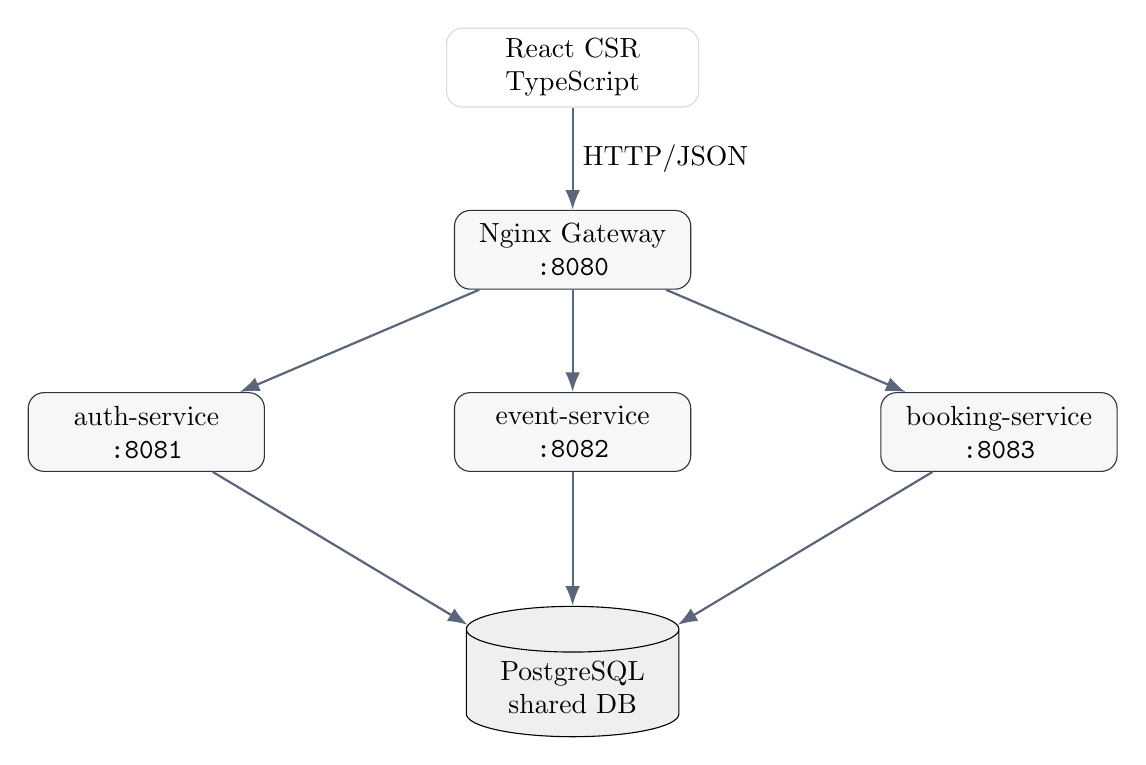
\begin{tikzpicture}[
  node distance=1.3cm,
  box/.style={draw=line, fill=white, rounded corners=2mm, minimum width=3.2cm, minimum height=1cm, align=center},
  service/.style={draw=brand, fill=soft, rounded corners=2mm, minimum width=3cm, minimum height=1cm, align=center},
  db/.style={draw=brandDark, fill=brand!8, cylinder, shape border rotate=90, aspect=0.28, minimum height=1.3cm, minimum width=2.7cm, align=center},
  arrow/.style={-{Latex[length=2.5mm]}, thick, draw=muted}
]
\node[box] (client) {React CSR\\TypeScript};
\node[service, below=of client] (gateway) {Nginx Gateway\\\code{:8080}};
\node[service, below left=1.3cm and 2.4cm of gateway] (auth) {auth-service\\\code{:8081}};
\node[service, below=1.3cm of gateway] (event) {event-service\\\code{:8082}};
\node[service, below right=1.3cm and 2.4cm of gateway] (booking) {booking-service\\\code{:8083}};
\node[db, below=1.7cm of event] (db) {PostgreSQL\\shared DB};
\draw[arrow] (client) -- node[right]{HTTP/JSON} (gateway);
\draw[arrow] (gateway) -- (auth);
\draw[arrow] (gateway) -- (event);
\draw[arrow] (gateway) -- (booking);
\draw[arrow] (auth) -- (db);
\draw[arrow] (event) -- (db);
\draw[arrow] (booking) -- (db);
\end{tikzpicture}
\caption{Systemarkitektur med gateway, services og fælles database}
\end{figure}

\subsection{Serviceopdeling}

Backend er delt op i tre services, fordi de har forskellige ansvarsområder.

\begin{table}[h]
\centering
\caption{Serviceopdeling}
\begin{tabularx}{\textwidth}{@{}L{3.2cm}Y@{}}
\toprule
Service & Ansvar \\
\midrule
\code{auth-service} & Registrering, login, logout, CSRF-bootstrap og opslag af aktuel bruger. Logisk ejer af \code{users}. \\
\code{event-service} & Eventkatalog, eventdetaljer, admin event lifecycle, sædegenerering og sædetilgængelighed. Logisk ejer af \code{events} og \code{seats}. \\
\code{booking-service} & Booking, multi-seat booking, annullering, brugerens bookinger, venteliste, admin bookingoversigt og gemte e-mailbeskeder. Logisk ejer af \code{bookings}, \code{waitlist\_entries} og \code{email\_outbox}. \\
\bottomrule
\end{tabularx}
\end{table}

\code{auth-service} håndterer registrering, login, logout, CSRF-token og opslag af den aktuelle bruger. Den logiske tabel for denne service er \code{users}. Auth-service kører også Flyway-migrationerne ved opstart, så databasen bliver sat op ét sted.

\code{event-service} håndterer eventkataloget og adminfunktioner for events. Det er her events oprettes, redigeres, publiceres, afpubliceres, annulleres og slettes. Servicen genererer også sæder ud fra en kapacitet og blokerer kapacitetsændringer, der ville fjerne bookede sæder. De logiske tabeller er \code{events} og \code{seats}.

\code{booking-service} er den eneste service, der skriver til bookingdelen. Den håndterer single-seat booking, multi-seat booking, annullering, brugerens egne bookinger, venteliste, admin bookingoversigt og gemte e-mailbeskeder. De logiske tabeller er \code{bookings}, \code{waitlist\_entries} og \code{email\_outbox}.

\subsection{Kursusdesignvalg}

Projektet kobler sig til kursusemnerne på følgende måde:

\begin{table}[h]
\centering
\caption{Kobling mellem kursusemner og projektvalg}
\begin{tabularx}{\textwidth}{@{}L{3cm}Y@{}}
\toprule
Kursusemne & Hvordan det er brugt i projektet \\
\midrule
Lektion 01--02 & Klient/server-applikation med browserklient, gateway, backend-services og database. \\
Lektion 03 og 12 & Login-cookie, CSRF-beskyttelse, bcrypt, validering, tilladte origins, roller og ensartede fejlbeskeder. \\
Lektion 05 & JSON bruges til request- og response-bodies i API'erne. \\
Lektion 06 & REST med ressource-URI'er, HTTP-verber og statuskoder. API'et sigter mod Richardson Level 2. \\
Lektion 07 & GraphQL blev valgt fra, fordi REST passer bedre til bookingflowets simple ressourcer og tydelige konfliktsvar. \\
Lektion 08 & CSR blev valgt, fordi appen er loginbaseret, interaktionstung og ikke afhænger af SEO. \\
Lektion 09--10 & Frontenden bruger React Router, TanStack Query, typed API-klient, responsive layout og komponenttests. \\
Lektion 13 & Projektet har backend-tests, frontend-tests, smoke script, concurrency script, baseline script og GitHub Actions. \\
\bottomrule
\end{tabularx}
\end{table}

\subsection{Databasedesign}

Databasen bruger UUID'er som primærnøgler og \code{TIMESTAMPTZ} til tidsstempler. Sæder har ikke en fast statuskolonne. I stedet beregnes ledige sæder ud fra sædelisten og de bookinger, der allerede findes. Det gør det sværere for systemet at vise en forkert sædestatus.

\begin{figure}[h]
\centering
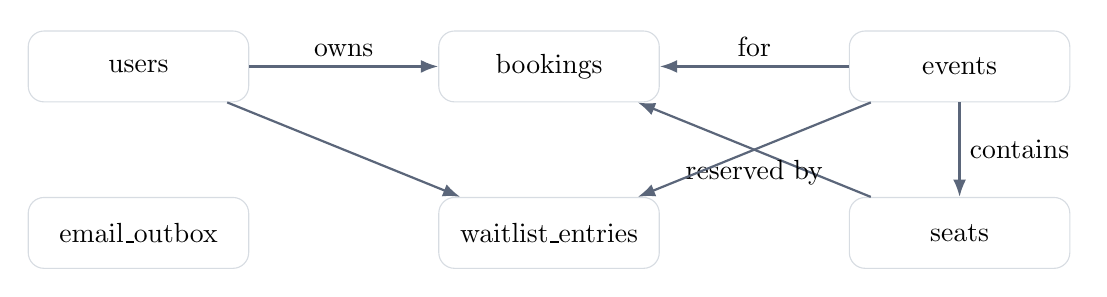
\begin{tikzpicture}[
  entity/.style={draw=line, fill=white, rounded corners=2mm, minimum width=2.8cm, minimum height=0.9cm, align=center},
  rel/.style={-{Latex[length=2.2mm]}, thick, draw=muted}
]
\node[entity] (users) {users};
\node[entity, right=2.4cm of users] (bookings) {bookings};
\node[entity, right=2.4cm of bookings] (events) {events};
\node[entity, below=1.2cm of events] (seats) {seats};
\node[entity, below=1.2cm of bookings] (waitlist) {waitlist\_entries};
\node[entity, below=1.2cm of users] (email) {email\_outbox};
\draw[rel] (users) -- node[above]{owns} (bookings);
\draw[rel] (events) -- node[above]{for} (bookings);
\draw[rel] (events) -- node[right]{contains} (seats);
\draw[rel] (seats) -- node[below]{reserved by} (bookings);
\draw[rel] (users) -- (waitlist);
\draw[rel] (events) -- (waitlist);
\end{tikzpicture}
\caption{Forenklet datamodel}
\end{figure}

\subsection{Concurrency-strategi}

Strategien mod dobbeltbooking har tre lag:

\begin{enumerate}
  \item Databasen tillader kun én booking per event og sæde.
  \item Booking-service gemmer bookinger i en transaktion.
  \item Hvis sædet allerede er taget, får brugeren et tydeligt konfliktsvar.
\end{enumerate}

\begin{lstlisting}[language=SQL,caption={Databasebegrænsning mod dobbeltbooking}]
CONSTRAINT uq_bookings_event_seat
    UNIQUE (event_id, seat_id)
\end{lstlisting}

\textbf{Hvorfor dette er vigtigt.} Hvis to brugere prøver at booke samme sæde på samme tid, er det ikke nok, at knappen bliver disabled i brugergrænsefladen. Backend og database skal også kunne stoppe den ene booking.

\subsection{Nginx gateway}

Nginx er systemets fælles indgang. Den viser frontend-filerne og sender API-kald videre til den rigtige backend-service. Gatewayen sætter også nogle basale sikkerhedsheadere i browseren. HTTPS er ikke en del af den lokale Docker Compose-opsætning.

Gatewayen begrænser også antallet af loginforsøg pr. IP. Det gør brute-force loginforsøg sværere.

\section{Implementation}

\subsection{Teknologivalg}

\begin{table}[h]
\centering
\caption{Teknologivalg}
\begin{tabularx}{\textwidth}{@{}L{3.4cm}Y@{}}
\toprule
Område & Teknologi \\
\midrule
Frontend & React 18, TypeScript, Vite, React Router, TanStack Query og Vitest. \\
Backend & Java 21, Spring Boot 3, Spring Security og Spring Validation. \\
Database & PostgreSQL 16 og Flyway. \\
Data access & Auth-service bruger Spring Data JPA. Event-service og booking-service bruger \code{NamedParameterJdbcTemplate}. \\
Sikkerhed & JWT i HttpOnly-cookie, bcrypt, CSRF-token og rollebaseret adgang. \\
Drift & Nginx, Docker, Docker Compose og GitHub Actions CI. \\
\bottomrule
\end{tabularx}
\end{table}

\subsection{Backend-implementation}

\subsubsection{Autentificering og autorisation}

Når en bruger logger ind, gemmes login-tokenet i en HttpOnly-cookie. Det betyder, at almindelig JavaScript-kode i browseren ikke kan læse tokenet. Fordi cookies automatisk sendes med requests, bruger systemet også en CSRF-token. Frontenden henter først en CSRF-token og sender den med, når den laver ændringer som login, booking eller annullering.

\begin{lstlisting}[language=Java,caption={JWT-cookie i auth-service}]
private ResponseCookie buildAuthCookie(String value, Duration maxAge) {
    return ResponseCookie.from(authCookieProperties.name(), value)
            .httpOnly(true)
            .secure(authCookieProperties.secure())
            .sameSite(authCookieProperties.sameSite())
            .path("/")
            .maxAge(maxAge)
            .build();
}
\end{lstlisting}

Rollebaseret adgangskontrol håndhæves i Spring Security med rollerne \code{USER} og \code{ADMIN}. Admin-routes er kun tilgængelige for brugere med \code{ADMIN}.

\subsubsection{Booking og concurrency-guard}

Booking-service finder selv brugerens id ud fra login-tokenet. Brugeren kan derfor ikke sende et andet bruger-id i requesten. Ved booking tjekker servicen først eventet og sædet. Derefter forsøger den at gemme bookingen. Ved multi-seat booking gemmes alle valgte sæder samlet. Hvis ét af sæderne allerede er taget, bliver hele bookingen afvist.

\begin{lstlisting}[language=Java,caption={Forenklet transaktionel multi-seat booking}]
@Transactional
public List<BookingReservation> reserveSeats(
        UUID userId, UUID eventId, List<UUID> seatIds) {
    EventRecord event = findBookableEvent(eventId);
    List<SeatRecord> seats = findSeats(eventId, uniqueSeatIds);
    List<BookingReservation> reservations = new ArrayList<>();

    for (SeatRecord seat : seats) {
        reservations.add(insertBooking(
            userId, eventId, seat.id(), seat.seatNumber()));
    }

    createEmail(findUserEmail(userId),
        "Booking confirmed: " + event.title(),
        "Your booking is confirmed.");
    return reservations;
}
\end{lstlisting}

\subsubsection{Venteliste og e-mailbeskeder}

Når et event er udsolgt, kan brugere tilmelde sig venteliste. Brugeren kan kun være på venteliste én gang per event, fordi databasen har en unik begrænsning på \code{(user\_id, event\_id)}.

E-mailbeskeder gemmes i \code{email\_outbox}. Systemet sender ikke rigtige e-mails, men gemmer de beskeder, der ville være sendt ved booking, annullering og ventelistenotifikation. Det er nok til demoen og kræver ikke en ekstern mailtjeneste.

\subsubsection{Event lifecycle}

Admin kan oprette, redigere, publicere, afpublicere, annullere og slette events. Events har statusværdierne \code{UNPUBLISHED}, \code{PUBLISHED} og \code{CANCELED}. Public event-listen viser kun publicerede og ikke-slettede events. Admin-dashboardet kan se alle ikke-slettede events.

Kapacitet kan øges ved at generere nye sæder. Reduktion blokeres, hvis det ville fjerne et allerede booket sæde. Sletning blokeres, hvis eventet har bookinger eller ventelisteindgange.

\subsection{Frontend-implementation}

Frontenden er organiseret i:

\begin{itemize}
  \item \filepath{pages/}: sidelogik for login, events, event detail, admin og egne bookinger.
  \item \filepath{components/}: genbrugelige komponenter som \code{AppShell}, \code{ProtectedRoute}, \code{AdminRoute} og \code{FormField}.
  \item \filepath{features/}: domænehooks til auth, events og bookings.
  \item \filepath{api/}: typed API-klient og TypeScript-typer.
\end{itemize}

Frontenden bruger React Router til siderne og TanStack Query til data fra serveren. Når brugeren fx booker eller annullerer, hentes data igen, så skærmen viser den nyeste status fra backend.

\subsection{Brugerflow i appen}

Det normale brugerflow starter på forsiden, hvor brugeren enten kan gennemse events eller logge ind. Forsiden forklarer kort, at systemet handler om eventbooking, sædevalg og concurrency-sikkerhed.

\flowimage{docs/pics/flow-01-landing.png}{Forside}{Forsiden samler de vigtigste indgange: eventlisten, login og oprettelse af konto.}

På login-siden kan brugeren enten skrive sine egne oplysninger eller vælge en demo-konto. Demo-knapperne gør det hurtigere at vise systemet under en præsentation uden at ændre selve loginflowet.

\flowimage{docs/pics/flow-02-login.png}{Login}{Login-siden viser demo-konti og almindelige loginfelter.}

Når brugeren er logget ind, vises eventlisten. Her kan brugeren søge i events og åbne et event for at se sæderne.

\flowimage{docs/pics/flow-03-events.png}{Eventliste}{Eventlisten viser publicerede events, ledige sæder og adgang til eventdetaljer.}

På eventdetaljesiden kan brugeren se status, samlet kapacitet, antal ledige sæder og sædekortet. Ledige sæder kan vælges, mens bookede sæder er låst.

\flowimage{docs/pics/flow-04-event-detail.png}{Eventdetaljer og sædekort}{Sædekortet viser tydeligt, hvilke sæder der er ledige, valgte eller bookede.}

Efter booking kan brugeren gå til \textit{My bookings}. Her vises brugerens aktive bookinger, og brugeren kan gå tilbage til eventet eller annullere bookingen, hvis eventet stadig ligger i fremtiden.

\flowimage{docs/pics/flow-05-my-bookings.png}{Mine bookinger}{Siden viser brugerens aktive reservationer og eventuelle ventelistepladser.}

\FloatBarrier

\section{Sikkerhed}

\subsection{Datakategorisering}

Vi brugte en simpel FIPS-199-inspireret vurdering af dataene:

\begin{table}[h]
\centering
\caption{Datakategorisering}
\begin{tabularx}{\textwidth}{@{}L{4cm}Y@{}}
\toprule
Data & Vurdering \\
\midrule
Loginoplysninger & Skal beskyttes, fordi de giver adgang til brugerkonti. Passwords gemmes derfor som hashes. \\
Brugerprofiler & Indeholder navn og e-mail og skal kun vises til den rigtige bruger eller admin. \\
Bookingdata & Skal være korrekte, fordi de viser hvem der ejer hvilke sæder. \\
Sædetilgængelighed & Er ikke hemmelig, men skal være korrekt, især når flere booker samtidigt. \\
Event-katalog & Er ikke følsomt indhold, men skal stadig være korrekt og troværdigt. \\
Admin-handlinger & Lav fortrolighed og høj integritet. Kun administratorer må udføre dem. \\
\bottomrule
\end{tabularx}
\end{table}

\subsection{Abuse cases og kontroller}

De vigtigste abuse cases og kontroller er:

\begin{table}[h]
\centering
\caption{Abuse cases og kontroller}
\begin{tabularx}{\textwidth}{@{}L{4cm}Y@{}}
\toprule
Risiko & Kontrol \\
\midrule
Credential stuffing & Nginx rate-limiter \code{POST /api/auth/login}. \\
XSS og token-tyveri & Login-tokenet gemmes i en HttpOnly-cookie, så det ikke kan læses direkte fra JavaScript. \\
CSRF & Requests der ændrer data, skal sende en CSRF-token med. \\
Dobbeltbooking & Databasen tillader kun én booking for samme sæde på samme event. \\
SQL injection & Databasekald bruger parametriserede queries i stedet for at bygge SQL med rå tekst fra brugeren. \\
Uautoriseret admin-adgang & Adminsider og admin-endpoints kræver rollen \code{ADMIN}. \\
Unødige tekniske detaljer i fejl & Brugeren får korte fejlbeskeder, og systemet viser ikke interne fejl fra backend. \\
\bottomrule
\end{tabularx}
\end{table}

\subsection{Gateway-sikkerhed}

Nginx tilføjer basale browserbeskyttelser, blandt andet mod clickjacking og mod at browseren gætter forkert på filtyper. Den begrænser også loginforsøg, så gentagne forsøg fra samme IP bremses.

HTTPS er ikke en del af den lokale Docker Compose-opsætning. I en rigtig produktionsopsætning bør TLS håndteres foran gatewayen eller direkte i gatewayen. Andre naturlige næste sikkerhedstiltag ville være bedre logning af admin-handlinger og automatisk tjek af sårbare dependencies.

\section{Monitorering og drift}

\subsection{Health checks}

Alle tre backend-services har et health endpoint. Docker Compose bruger det til at se, om en service er klar, før gatewayen starter.

\begin{lstlisting}[caption={Eksempel på Docker Compose health check}]
healthcheck:
  test:
    ["CMD-SHELL",
     "curl -fsS http://localhost:8081/actuator/health >/dev/null || exit 1"]
  interval: 10s
  timeout: 5s
  retries: 12
\end{lstlisting}

\subsection{Loginbegrænsning}

Nginx begrænser loginforsøg pr. IP:

\begin{lstlisting}[caption={Login rate limiting i Nginx}]
limit_req_zone $binary_remote_addr zone=login_limit:10m rate=20r/m;

location = /api/auth/login {
  limit_req zone=login_limit burst=10 nodelay;
  proxy_pass http://auth-service:8081;
}
\end{lstlisting}

\subsection{Måling af svartider}

\code{scripts/measure-baseline.mjs} måler responstider for:

\begin{itemize}
  \item frontendens første HTML-response
  \item \code{GET /api/events}
  \item \code{GET /api/events/\{id\}}
  \item \code{GET /api/events/\{id\}/seats}
\end{itemize}

Disse målinger giver et udgangspunkt, som kan bruges, hvis man senere vil optimere performance.

\subsection{Fremtidig monitorering}

Projektet har health checks og scripts, men ikke et fuldt monitoreringssystem. I en større driftssituation ville næste trin være fælles logs, simple alarmer og løbende målinger af svartider og fejl.

\section{Afprøvning}

\subsection{Backend-tests}

Backend-tests er skrevet med JUnit 5, Spring Boot Test og Testcontainers. De tester blandt andet:

\begin{itemize}
  \item auth-flow med registrering, login, logout, \code{/me} og CSRF
  \item event-oprettelse, statusændringer, kapacitetsændring og adgangskontrol
  \item booking, multi-seat booking, cancellation, waitlist og admin bookingoversigt
  \item databaseintegritet og concurrency-relevante fejlscenarier
\end{itemize}

Testcontainers kræver Docker-adgang i testmiljøet. Derfor er GitHub Actions det bedste sted at dokumentere, at hele backend-testpakken kan køre.

\subsection{Frontend-tests}

Frontend-tests med Vitest dækker blandt andet login, registrering, eventlisten, eventdetaljer, beskyttede sider, admin-sider, booking-hooks, venteliste, email outbox og CSRF-håndtering i API-klienten.

\subsection{Smoke tests og scripts}

Projektet har tre vigtige scripts:

\begin{table}[h]
\centering
\caption{Smoke tests og scripts}
\begin{tabularx}{\textwidth}{@{}L{4.4cm}Y@{}}
\toprule
Script & Formål \\
\midrule
\code{smoke-test.mjs} & Går igennem et samlet bruger- og admin-flow mod en kørende app. \\
\code{concurrency-demo.mjs} & Lader to brugere forsøge at booke samme sæde og kontrollerer, at kun én booking lykkes. \\
\code{measure-baseline.mjs} & Måler svartider for forsiden og de vigtigste event-API'er. \\
\bottomrule
\end{tabularx}
\end{table}

\subsection{Continuous Integration}

GitHub Actions workflowet kører ved push og pull request til \code{main}. Det har to jobs:

\begin{itemize}
  \item Backend: Java 21 og \code{mvn -B test}
  \item Frontend: Node 22, \code{npm ci}, \code{npm test -- --run} og \code{npm run build}
\end{itemize}

Der er CI, men ikke automatisk deployment. Deployment sker manuelt via Docker Compose-runbook.

\section{Idriftsættelse}

\subsection{Containeriseringsstrategi}

Hele systemet køres med Docker Compose. Backend-services bygges i Docker med Maven og køres derefter som Java-applikationer. Frontenden bygges ind i gateway-containeren og serveres som statiske filer fra Nginx.

\subsection{Docker Compose-opsætning}

Compose-filen definerer fem services: \code{postgres}, \code{auth-service}, \code{event-service}, \code{booking-service} og \code{gateway}. PostgreSQL starter først. Derefter starter backend-services, og til sidst starter gatewayen, når services er klar.

Gatewayens host-port kan ændres med \code{GATEWAY\_PORT}. Det gør det muligt at køre projektet samtidig med en anden lokal app:

\begin{lstlisting}[language=bash,caption={Kør projektet på port 3000}]
GATEWAY_PORT=3000 docker compose -f infrastructure/docker-compose.yml up --build
\end{lstlisting}

\subsection{Deploymentmålplatform}

Målplatformen er en Debian 12-VM med Docker og Docker Compose. Repoet indeholder en runbook i \filepath{docs/deployment.md}. Den beskriver, hvordan man installerer Docker, kloner repoet, sætter miljøvariabler og starter systemet.

Efter deployment kan man gemme bevis i \filepath{docs/deployment-evidence.md}, fx Docker-version, containerstatus, health checks og output fra smoke-test og concurrency-demo.

\subsection{Miljøer og konfiguration}

Vi skelner mellem fire miljøer:

\begin{table}[h]
\centering
\caption{Miljøer}
\begin{tabularx}{\textwidth}{@{}L{3.4cm}Y@{}}
\toprule
Miljø & Formål \\
\midrule
Lokal udvikling & Udvikling og manuel test med Docker Compose eller frontend dev server. \\
CI & Automatisk test og build i GitHub Actions. \\
Staging/demo & Kørende Docker Compose-stack til integrationstest og demo. \\
Debian VM & Målplatform for den endelige deployment-evidence. \\
\bottomrule
\end{tabularx}
\end{table}

Miljøspecifikke værdier som database-login, JWT-secret, allowed origins, cookie-indstillinger og gateway-port sættes via environment variables.

\section{Konklusion}

Vi har udviklet et distribueret event-bookingsystem med React CSR-frontend, tre Spring Boot-services, Nginx gateway, PostgreSQL, Flyway-migrationer, Docker Compose og CI. Systemet er ikke kun en prototype med statiske data; det har rigtige brugerflows, databasepersistens, login, rollebaseret adgang, adminfunktioner, venteliste og bookinglogik.

Den vigtigste del af projektet er concurrency-løsningen for sædebooking. Ved at kombinere transaktionelle writes med en unik databasebegrænsning kan systemet afvise dobbeltbooking, selv når to brugere forsøger at booke samme sæde samtidigt. Det er også derfor, concurrency-demoen er en central del af projektet: den viser, at løsningen ikke kun virker i brugergrænsefladen, men også når to requests rammer backend næsten samtidigt.

Projektet viser også de valg, som kurset har fokuseret på. Vi bruger JSON og REST frem for GraphQL, fordi bookingflowet passer godt til simple endpoints og tydelige HTTP-statuskoder. Vi bruger CSR, fordi applikationen primært er loginbaseret og interaktiv. Vi bruger Docker Compose og en gateway, så systemet kan startes samlet og testes som en helhed.

Derudover har projektet et praktisk sikkerhedsniveau med JWT i HttpOnly-cookie, CSRF-beskyttelse, bcrypt, rollebaseret adgang, validering, Nginx security headers og begrænsning af loginforsøg. Systemet er dokumenteret med API-kontrakter, Postman collection, deployment-runbook, verification scripts og CI.

Samlet set viser projektet, at vi kan designe, implementere, teste og dokumentere en full-stack-applikation med reel kompleksitet. Projektet har stadig oplagte næste skridt, fx rigtig e-mailudsendelse, audit logging og en mere komplet produktionsopsætning, men de vigtigste krav for kurset er dækket: full-stack arkitektur, REST/JSON-kommunikation, sikkerhed, test, deploymentbarhed og håndtering af concurrent access til en delt ressource.

\section{Litteraturliste}

\begin{enumerate}
  \item Leonard Richardson, \textit{Richardson Maturity Model}, \url{https://martinfowler.com/articles/richardsonMaturityModel.html}
  \item Roy T. Fielding, \textit{Architectural Styles and the Design of Network-based Software Architectures}, University of California, Irvine, 2000.
  \item Spring Boot Reference Documentation, \url{https://docs.spring.io/spring-boot/}
  \item React Documentation, \url{https://react.dev/}
  \item PostgreSQL 16 Documentation, \url{https://www.postgresql.org/docs/16/}
  \item Docker Documentation, \url{https://docs.docker.com/}
  \item Nginx Documentation, \url{https://nginx.org/en/docs/}
  \item NIST FIPS 199, \textit{Standards for Security Categorization of Federal Information and Information Systems}, \url{https://csrc.nist.gov/publications/detail/fips/199/final}
  \item OWASP, \textit{Cross-Site Request Forgery Prevention Cheat Sheet}, \url{https://cheatsheetseries.owasp.org/cheatsheets/Cross-Site_Request_Forgery_Prevention_Cheat_Sheet.html}
  \item Vite Documentation, \url{https://vite.dev/}
\end{enumerate}

\end{document}
